\usepackage{xspace}
\newcommand{\ps}{phylesystem\xspace}
\newcommand{\otol}{Open Tree of Life\xspace}
\newcommand{\nexson}{otNexSON\xspace}
\newcommand{\js}{JavaScript\xspace}
\newcommand{\authorswaffil}{Emily Jane McTavish,$^{1}$
 James Pettengill$^{2}$, Steve Davis$^{2}$, Hugh Rand$^{2}$, Errol Strain$^{2}$, Marc Allard$^{2}$,
 Ruth E. Timme$^{2}$
}
\newcommand{\affil}{$^{1}$ Department of Ecology and Evolutionary Biology, University of Kansas, Lawrence KS, USA\\
$^{2}$ Center for Food Safety and Nutrition, Food and Drug Administration, College Park, MD\\
}

\begin{document}
\firstpage{1}
\mytitle{Tree to Reads}{TreeToReads - a pipeline for simulating raw reads from phylogenies}

\myauthor{McTavish \textit{et~al}}{\authorswaffil}
\myaddress{\affil}
\history{Received on XXXXX; revised on XXXXX; accepted on XXXXX}
\editor{Associate Editor: XXXXXXX}
\maketitle
\posttitle{\authorswaffil}{\affil}


\begin{abstract}
\textbf{Summary:}
Using genome-wide single nucleotide polymorphism (SNP)-based methods for tracking pathogens has become standard practice in academia and public health agencies.
Multiple computational approaches call variants by mapping short read data against a reference genome, filtering those variants for quality, 
then concatenating them into a sequence matrix for down-stream phylogenetic analysis.
However, despite our knowledge of the parameters that affect whether a SNP is called, 
we lack methods for determining the effects of read mapping choices on whether the correct tree has been recovered.
To resolve this problem, we offer a program, TreeToReads, which can generate raw read data from mutated genomes simulated under a known phylogeny.
This simulation pipeline allows direct comparisons of simulated and observed data to the same reference genome,
and therefore can be used to test the phylogenetic effects of distance to that reference genome.
At each step of these simulations, researchers can vary parameters of interest (e.g., topology, model of sequence evolution, and read coverage)
to assess the robustness of a given result. Such critical assessments of the accuracy and robustness of analytical pipelines are essential to progress in both research and applied settings.

\textbf{Availability and implementation:}
Source code, examples, and a tutorial are available at \url{https://github.com/snacktavish/TreeToReads}. 

\textbf{Contact:} ejmctavish@gmail.com
\textbf{Supplementary information:}
Input and output files for the case study are available in the online supplementary information.
\end{abstract}

\section*{Introduction}
Whole genome sequencing now allows us to see details sufficient to differentiate among genetic samples that differ by only a few single nucleotide polymorphisms (SNPs).
Such small differences can be indicative of recent divergences that are the first increments of evolutionary change.
However, especially in cases where estimates of ancestry rely on a handful of data points, 
it is particularly important to ensure that our methods for ascertaining these variable sites from sequence data are validated and free from bias.
As the resulting phylogenetic trees may used by public heath agencies to make regulatory decisions (e.g. identifying a source in a foodborne outbreak \citep{hoffmann_tracing_2015}),
or becoming the basis for enforcement or legal actions, we need ways to ensure inferred trees are correct. 

SNP-calling biases can be caused by various factors, 
including genotyping of single nucleotides which are polymorphic in a subset of the population \citep{mctavish_how_2015}, 
missing data cutoffs resulting in preferential inclusion of loci evolving at lower rates \citep{huang_unforeseen_2014} and those related to read mapping due to choice of reference genome \citep{bertels_automated_2014},
filter artifacts \citep{li_toward_2014} and different mapping algorithms \citep{pightling_choice_2014}. 
Mis-estimation can be exacerbated by interaction between these dataset biases and analysis choices; 
for example using a model of evolution developed for sequence data on a panel of exclusively variable sites \citep{lewis_likelihood_2001} 
or choosing an inappropriate model of evolution \citep{sullivan_are_1997}. Despite the sheer quantities of genomic data, 
it is possible that these types of biases could affect phylogenetic conclusions and, if systematic, inappropriate methods may converge to an incorrect result with high bootstrap confidence. 
In order to adopt data analysis pipelines for the regulatory environment it is necessary to understand these biases and validate their use. 
Without in silico modeling food safety scientists would have to rely on benchmark datasets where the “truth” can never be truly known.


Here, we present TreeToReads (TreeToReads), a software tool to simulate realistic patterns of sequence variation across phylogenies 
in order to assess the robustness of evolutionary inferences from whole genome data to potential biases in the data collection and analysis pipeline. 

There are two key aspects of TreeToReads that together differentiate it from existing simulation alternatives.
Firstly, the variable sites follow a user specified phylogeny.
Secondly, those variable sites are placed in the context of an observed or `anchor' genome, which is represented as tip of that phylogeny.
This combination allows for direct comparisons of read mapping between observed and simulated reads, 
and make TreeToReads appropriate for testing effects of distance to a reference genome on phylogenetic inference from genomic data.
The `anchor genome' can be used as a reference genome for read mapping, or mapping can be tested against other empirically observed genomes.
In the latter case, real evolutionary history separates the reference and the simulated data.
Simulated sequences where a known genome is a tip on the tree makes these direct comparisons for testing reference genome effects, 
and is not possible using existing simulation software.

\begin{figure*}[trees]
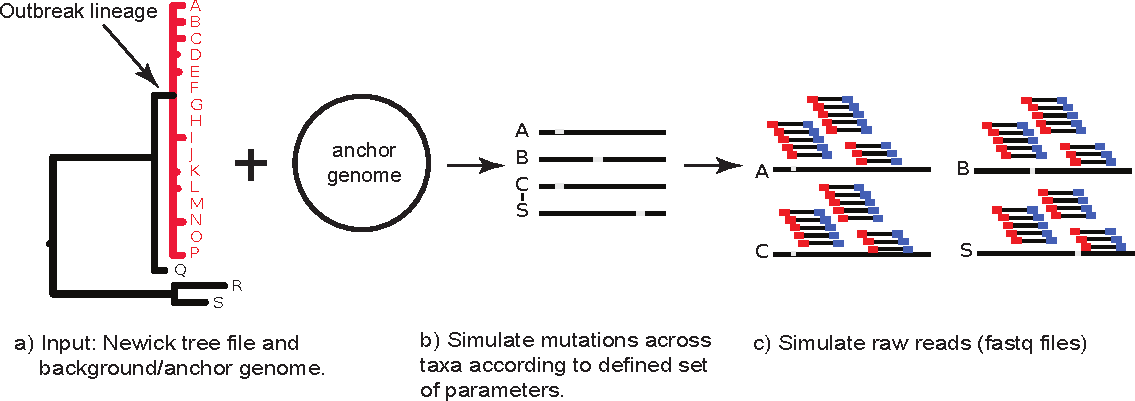
\includegraphics[width=6.5in]{TTR-figure}
\caption{Schematic of the TreeToReads procedure}
\label{scheme}
\end{figure*}

\section*{Methods}
The TreeToReads pipeline generates short read data from genomes simulated along an input phylogeny. 
The software is written in Python and requires two input files - a phylogeny with branch lengths and a FASTA formatted genome sequence which serves as the `anchor genome'.
The user specifies parameter settings (e.g., number of variable sites to simulate and nucleotide substitution model parameters) in a configuration file.
The branch lengths of the user provided phylogeny determine the relative number of mutations on each branch 
and the probability that a single site is affected by multiple mutational events.
To account for the ascertainment bias inherent in estimating phylogenies from panels of variable sites, 
the total number of variable sites is determined by a user input parameter, not the branch lengths.
The pipeline uses seq-gen \citep{rambaut_seq-gen:_1997} to simulate the variable sites specified in the configuration file along the input phylogeny.
Phylogeny formats are standardized using DendroPy \cite{sukumaran_dendropy:_2010}.
These sites are then distributed across the anchor genome.
The locations for mutations are either drawn from a uniform distribution,
or clustered according to parameters of an exponential distribution specified in the configuration file. 
This procedure creates an output folder for each tip in the tree that contains the simulated genomes (FASTA files).
A user specified tip will consist of the input anchor genome without any mutations.
Using these simulated genomes, 
TreeToReads calls the read simulation software, ART, \citep{huang_art:_2012} to generate Illumina MiSeq paired-end reads.
The user can apply a default sequence error model, or use the configuration file to specify an error model generated for observed data.
TreeToReads currently supports automated generation of Illumina paired end reads.
For other read types, the simulated genome files may be used outside of TreeToReads with any ART parameter configuration. 
Alternatively, if RAD-seq like data are desired other raw-read generators such as SimRAD \citep{lepais_simrad:_2014} can be used. 
If ART is invoked in TreeToReads the program will output a fastq folder containing directories labeled with the names of each tip from the 
simulation tree within which the simulated reads in .fastq.gz and .sam format are deposited. 
A file with the location and nucleotide state of each mutation within each tip is also provided.


\section{Case Study}
To demonstrate TreeToReads, we tested the effects of sequence coverage and choice of reference genome on SNP calling and recovery of a phylogeny.
\emph{(TODO: Umm, we didn't actually do an alt reference yet, but I think it would be worthwhile to map to a random Salmonella Enterica, because that is the thing you really can't do with other simulation software!)}
As a case study we used an observed phylogeny from ten \emph{Salmonella enterica} Bareilly sequences associated with a 2010 outbreak \citep{hoffmann_tracing_2015}.
We were interested in determining whether under simulated conditions we were able to capture the phylogenetic split that distinguishes the isolates belonging to the outbreak from isolates which are not part of the outbreak.
We used a completed \emph{Salmonella enterica} genome (CFSAN000189, GenBank: CP006053.1) as the anchor sequence, and simulated 150 variable sites under the GTR model.
SNP's were clustered with locations for 20\% drawing from an exponential distribution with a 125bp mean, based on the locations of variable sites in the observed sequence data.
The read error profile was generated from the observed outbreak sequence data.
We simulated data sequence coverage settings an average of 1, 5, 15, and 30 reads at each site. 
We analyzed the resulting four short read datasets with the Food and Drug Administration, Center for Food Safety And Nutritions SNP pipeline to identify SNPS in each simulated dataset \citep{davis_cfsan_2015}.
\emph{(MORE ON PIPELINE?)}
Reads were mapped to either the anchor genome, or a more distant reference (???? LT2?).
The distant reference genome is ??? \% diverged from the anchor genome.
We inferred the phylogeny for each set using RAxML under the ASC\_GTRCAT model which corrects for including only variable sites  \citep{stamatakis_raxml_2014} .
We found that when using the anchor genome as a reference, only at a average coverage of 1 read per site was it not possible to correctly infer the lineage leading to the outbreak clade.
At higher coverage levels the correct phylogeny was consistently inferred.
When mapping reads to a more distant reference genome \emph{(????)}.
\emph{comparison results?}
This simple test case demonstrates an application of TreeToReads to analysing the effects of coverage and distance
to reference genome on phylogenetic inference from next generation sequencing reads.

\section*{Comparison to existing software}
Many software tools exist for simulating sequence data,
but no existing tools unite both phylogenetic realtionships and observed genomic sequences.
TreeToReads is designed to test the effects of distance to a reference genome on phylogenetic inference.
In addition, TreeToReads provides a pipeline to simulate next-gen sequencing reads from a phylogenetic tree using an observed error model.
Using an anchor genome as a tip in the simulated tree means that simulated and empirical data can be mapped to the same reference genome,
providing direct comparisons of inferences.
In addition, that reference genome does not need to be the anchor genome on which the simulations are based.
If a different reference is used, the biological evolution separating the anchor genome from the reference genome 
includes real evolutionary processes affecting read mapping to genomes in a testable framework. %TODO IGGHHH

SeqGen \citep{rambaut_seq-gen:_1997} which is used to generate the variable sites in the TreeToReads pipeline, uses the full model generalized time reversible model of evolution specified.
However, on its own, SeqGen generates random sequences based on the model of evolution and therefore does not incorporate observed genomic context.
Reads from these simulated genomes cannot be mapped to an observed reference genome.
This is also true for other simulators of more complex evolutionary processes, such as Indelible \citep{fletcher_indelible:_2009} and SWGE \citep{arenas_simulation_2014}.
These simulators include complex evolutionary processes not simulated in TreeToReads, such as indels and recombination across lineages.
While these processes can be very important for accuracy of inference in phylogenetic questions at deeper timescales, they are not drivers of variation in closely related outbreak lineages (TODO: REF?).
Other sequence simulation software such as ALF \citep{dalquen_alfsimulation_2012}, and Indel Seq-gen \citep{strope_indel-seq-gen:_2007}
can accept as input a genome representing the root of the phylogeny.
However, in empirical data the reference genome is not an ancestor - it is always a present day relative.
Anchoring an observed genome to a tip in a tree using TreeToReads allows us to test choices about selection 
of reference genomes in a way that is directly comparable to empirical data.


\section*{Conclusions}
Existing genomic simulation software lack a phylogenetic perspective in simulation testing of assembly and alignment tools. 
TreeToReads allows researchers to test the joint effects of multiple parameter values
on the ability of any analysis pipeline to recover the signal and infer the correct tree. 
Simulating data that spans these parameters can validate methods for reconstructing phylogenies directly from short-read data, 
which is especially useful for public health agencies using these methods to track emerging pathogens. 


%%Don't forget to thank Torsten and Lee Katz
\bibliography{note}
\end{document}
